\begingroup
\renewcommand{\baselinestretch}{1}\selectfont
% Local, reusable vector figure styles. Units are centimetres.
\tikzset{
 thesis block/.style={draw=black,line width=.65pt,align=center,inner sep=5pt,font=\sffamily\fontsize{10}{12}\selectfont},
 thesis hw/.style={thesis block,fill=black!9},
 thesis sw/.style={thesis block,fill=white},
 thesis memory/.style={thesis block,double,double distance=1pt,fill=black!3},
 thesis arrow/.style={->,>=stealth,line width=.7pt},
 thesis transfer/.style={<->,>=stealth,line width=.7pt},
 thesis note/.style={align=center,font=\sffamily\fontsize{9}{11}\selectfont,inner sep=3pt},
 thesis title/.style={thesis note,font=\sffamily\bfseries\fontsize{10}{12}\selectfont}
}

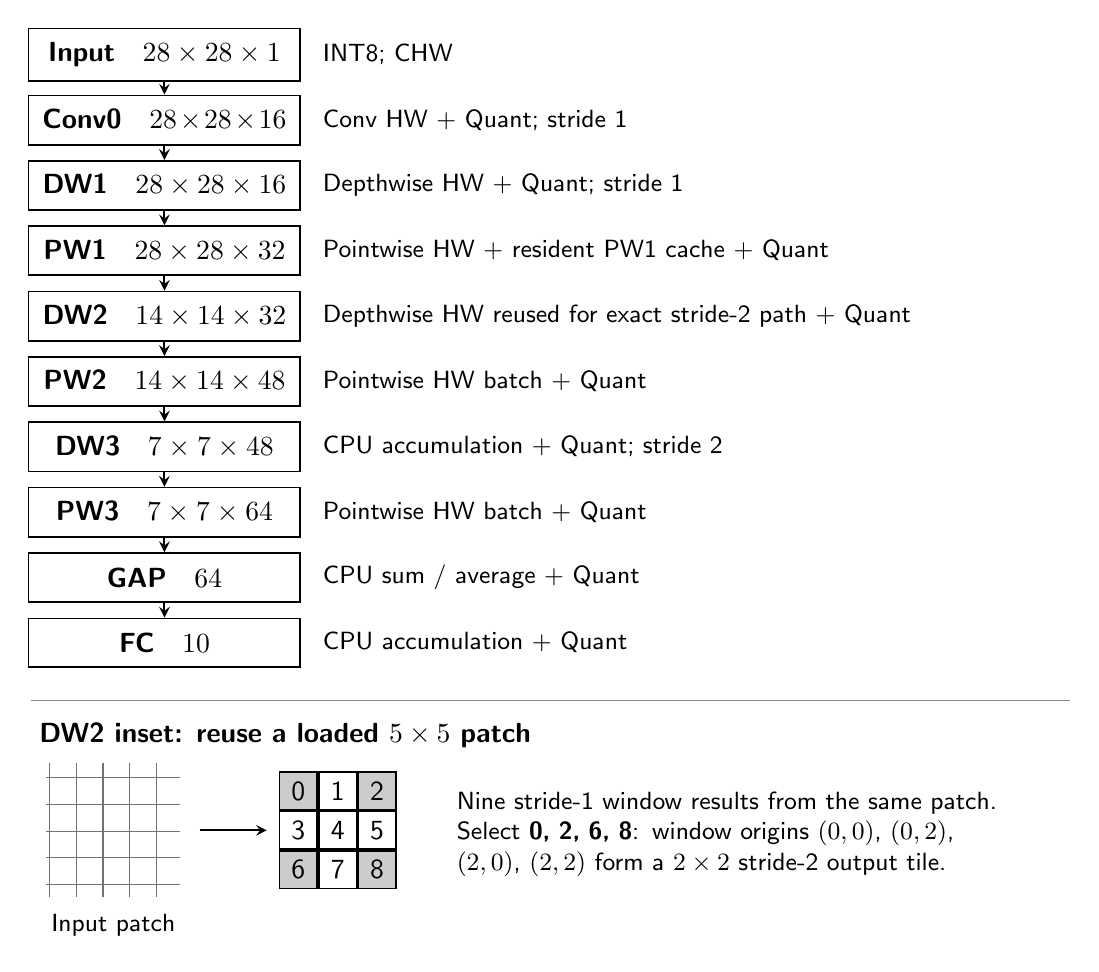
\begin{tikzpicture}[x=1cm,y=1cm]
\node[thesis block,text width=3.1cm,minimum height=.62cm] (n0) at (1.8,0.0) {\textbf{Input}\quad $28\times28\times1$};
\node[thesis note,anchor=west,align=left,text width=9.2cm] at (3.7,0.0) {INT8; CHW};
\node[thesis block,text width=3.1cm,minimum height=.62cm] (n1) at (1.8,-0.83) {\textbf{Conv0}\quad $28\times28\times16$};
\node[thesis note,anchor=west,align=left,text width=9.2cm] at (3.7,-0.83) {Conv HW + Quant; stride 1};
\draw[thesis arrow] (n0)--(n1);
\node[thesis block,text width=3.1cm,minimum height=.62cm] (n2) at (1.8,-1.66) {\textbf{DW1}\quad $28\times28\times16$};
\node[thesis note,anchor=west,align=left,text width=9.2cm] at (3.7,-1.66) {Depthwise HW + Quant; stride 1};
\draw[thesis arrow] (n1)--(n2);
\node[thesis block,text width=3.1cm,minimum height=.62cm] (n3) at (1.8,-2.4899999999999998) {\textbf{PW1}\quad $28\times28\times32$};
\node[thesis note,anchor=west,align=left,text width=9.2cm] at (3.7,-2.4899999999999998) {Pointwise HW + resident PW1 cache + Quant};
\draw[thesis arrow] (n2)--(n3);
\node[thesis block,text width=3.1cm,minimum height=.62cm] (n4) at (1.8,-3.32) {\textbf{DW2}\quad $14\times14\times32$};
\node[thesis note,anchor=west,align=left,text width=9.2cm] at (3.7,-3.32) {Depthwise HW reused for exact stride-2 path + Quant};
\draw[thesis arrow] (n3)--(n4);
\node[thesis block,text width=3.1cm,minimum height=.62cm] (n5) at (1.8,-4.1499999999999995) {\textbf{PW2}\quad $14\times14\times48$};
\node[thesis note,anchor=west,align=left,text width=9.2cm] at (3.7,-4.1499999999999995) {Pointwise HW batch + Quant};
\draw[thesis arrow] (n4)--(n5);
\node[thesis block,text width=3.1cm,minimum height=.62cm] (n6) at (1.8,-4.9799999999999995) {\textbf{DW3}\quad $7\times7\times48$};
\node[thesis note,anchor=west,align=left,text width=9.2cm] at (3.7,-4.9799999999999995) {CPU accumulation + Quant; stride 2};
\draw[thesis arrow] (n5)--(n6);
\node[thesis block,text width=3.1cm,minimum height=.62cm] (n7) at (1.8,-5.81) {\textbf{PW3}\quad $7\times7\times64$};
\node[thesis note,anchor=west,align=left,text width=9.2cm] at (3.7,-5.81) {Pointwise HW batch + Quant};
\draw[thesis arrow] (n6)--(n7);
\node[thesis block,text width=3.1cm,minimum height=.62cm] (n8) at (1.8,-6.64) {\textbf{GAP}\quad $64$};
\node[thesis note,anchor=west,align=left,text width=9.2cm] at (3.7,-6.64) {CPU sum / average + Quant};
\draw[thesis arrow] (n7)--(n8);
\node[thesis block,text width=3.1cm,minimum height=.62cm] (n9) at (1.8,-7.47) {\textbf{FC}\quad $10$};
\node[thesis note,anchor=west,align=left,text width=9.2cm] at (3.7,-7.47) {CPU accumulation + Quant};
\draw[thesis arrow] (n8)--(n9);

\draw[black!45] (.1,-8.2)--(13.3,-8.2);
\node[thesis title,anchor=west] at (.1,-8.65) {DW2 inset: reuse a loaded $5\times5$ patch};
\draw[step=.34,black!55] (.3,-10.7) grid (2,-9);
\node[thesis note] at (1.15,-11.05) {Input patch};
\draw[thesis arrow] (2.25,-9.85)--(3.1,-9.85);
\foreach \r in {0,1,2}{\foreach \c in {0,1,2}{
 \pgfmathtruncatemacro{\idx}{3*\r+\c}
 \ifnum\idx=0\def\shade{20}\else\ifnum\idx=2\def\shade{20}\else\ifnum\idx=6\def\shade{20}\else\ifnum\idx=8\def\shade{20}\else\def\shade{0}\fi\fi\fi\fi
 \node[thesis block,fill=black!\shade,minimum size=.48cm,inner sep=0pt] at ({3.5+.5*\c},{-9.35-.5*\r}) {\idx};
}}
\node[thesis note,text width=7.3cm,align=left,anchor=west] at (5.4,-9.9) {Nine stride-1 window results from the same patch.\\Select \textbf{0, 2, 6, 8}: window origins $(0,0)$, $(0,2)$,\\$(2,0)$, $(2,2)$ form a $2\times2$ stride-2 output tile.};

\end{tikzpicture}
\endgroup
